\documentclass[handout]{beamer}
\usepackage{beamerthemesplit}
\usepackage{pgfpages}
\usepackage{verbatim}

\usepackage{tikz}
\usetikzlibrary{arrows,%
                shapes,positioning}

\tikzstyle{vertex}=[circle,fill=black!25,minimum size=20pt,inner sep=0pt]
\tikzstyle{selected vertex} = [vertex, fill=red!24]
\tikzstyle{edge} = [draw,thick,-]
\tikzstyle{weight} = [font=\small]
\tikzstyle{selected edge} = [draw,line width=5pt,-,red!50]
\tikzstyle{ignored edge} = [draw,line width=5pt,-,black!20]

\newcommand{\field}[1]{\mathbb{#1}} %requires amsfonts

\usetheme{Antibes}
\usecolortheme{beaver}
\title[Higher Order Composite Field Decomposition]{Composite Field Decomposition for Higher Order S-Boxes}

\usepackage{mathptmx}
\usepackage[scaled=.90]{helvet}
\usepackage{courier}
\usepackage[T1]{fontenc}

%\pgfpagesuselayout{4 on 1}[letterpaper,border shrink=5mm]

\institute[RIT]{}
\date{\today}
%\subtitle{}
\author{Christopher A. Wood}
%\institute[]{}
\date{\today}

\begin{document}

%%%%%
%%
%% Resource link: http://www.math-linux.com/spip.php?article77
%%
%%%%

\begin{frame}
	\titlepage
\end{frame}

\begin{frame}
	\frametitle{Agenda}
	\tableofcontents
\end{frame}

\section{Composite Fields}
\begin{frame}
\begin{itemize}
	\item \emph{Q: Why use combinational logic?}
	\item A: Optimize hardware area of SubBytes operation on memory-constrained platforms (i.e. where LUTs are not acceptable implementations)
	\item \emph{Q: How are composite fields useful?}
	\item A: The multiplicative inverse calculation is the most expensive operation - using composite fields helps us reduce the gate-level complexity of this operation.
\end{itemize}
\end{frame}

\begin{frame}
	\frametitle{Composite Fields}
	A \emph{composite field} is a pair 
	\begin{align*}
	& \{GF(2^n), Q(y) = y^n + \sum_{i=0}^{n-1}q_iy^i, q_i \in GF(2)\} \\
	& \{GF((2^n)^m), P(x) = x^m + \sum_{i=0}^{m-1}p_ix^i, p_i \in GF(2^n)\},
	\end{align*}
	where $GF(2^n)$ is constructed from $GF(2)$ by $Q(y)$, and $GF((2^n)^m)$ is
	constructed from $GF(2^n)$ by $P(x)$. Also, $GF((2^n)^m)$ is a degree $m$ extension
	of $GF(2^n)$.
\end{frame}

\section{Common AES Composite Field Extensions}
\begin{frame}
Research has systematically examined all composite field extensions for $GF(2^8)$, seeking to minimize the area...
\begin{align*}
GF(2^4) - GF((2^4)^2) \\
GF(2^2) - GF((2^2)^4) \\
GF(2^2) - GF((2^2)^2) - GF(((2^2)^2)^2)
\end{align*}
\begin{itemize}
	\item The irreducible polynomial cannot exceed the degree of the extension $\to$ degree two extensions have the smallest number of irreducible polynomials!
	\item A systematic evaluation must check all tower field extensions \textbf{and} all irreducible polynomials.
	\item \textbf{Thesis Work:} Generate all possible irreducible polynomials for all tower field extensions.
\end{itemize}
\end{frame}

\section{Tower Field Isomorphic Functions}
\begin{frame}
The isomorphic functions are constructed as follows (assume we're constructing a function for mapping $GF(2^{nm}) \to GF((2^n)^m)$):
\begin{itemize}
	\item Find two generators $\alpha$ and $\beta$ ($\alpha \in GF(2^{nm})$ and $\beta \in GF((2^n)^m)$), where $\alpha$ and $\beta$ are roots of the same primitive irreducible polynomial. 
	\item Map $\alpha^k \to \beta^k$ for $1 \leq k \leq 2^{nm}$ (mapping basis elements of $GF(2^{nm}) \to GF((2^n)^m)$). If the mapping doesn't hold group homomorphism, find the next generator $\beta$ and repeat.
\end{itemize}
\end{frame}

\section{AES Combinational Implementations}
\begin{frame}
	\frametitle{AES Combinational Implementations}
	Every element in a field $GF(2^{nm})$ can be represented by a polynomial with coefficients from $GF(2^n)$ using 
	an irreducible polynomial of the form $x^2 + Ax + B$ (we assume $m = 2$). Thus, if $\alpha \in GF(2^{nm})$, and $\alpha = bx + c$, where $b,c \in GF(2^n)$, then:
	\begin{align*}
	\alpha^{-1} = (bx + c)^{-1} = b(b^2B + bcA + c^2)^{-1} + (c + bA)(b^2B + bcA + c^2)^{-1}
	\end{align*}
	Now we compute the inverse over $GF(2^n)$! We can also play with $A$ and $B$ to simplify the isomorphic mapping.
\end{frame}

\begin{frame}
	\frametitle{Isomorphic Functions}
	Once an isomorphic function $\delta$ is defined it can be implemented in hardware using constraint matrices.\\

	\textbf{Example:} A $\delta$ from $GF(2^8) \to GF((2^4)^2)$ (using the irreducible polynomial $p(x) = x^8 + x^4 + x^3 + x^2 + 1$) can be defined as follows:
	\begin{align*}
	\delta =  \left( \begin{array}{cccccccc}
1 & 1 & 0 & 0 & 0 & 0 & 1 & 0 \\
0 & 1 & 0 & 0 & 1 & 0 & 1 & 0 \\
0 & 1 & 1 & 1 & 1 & 0 & 0 & 1 \\
0 & 1 & 1 & 0 & 0 & 0 & 1 & 1 \\
0 & 1 & 1 & 1 & 0 & 1 & 0 & 1 \\
0 & 1 & 1 & 1 & 1 & 0 & 1 & 1 \\
0 & 0 & 0 & 0 & 0 & 1 & 0 & 1 \end{array} \right)
	\end{align*}
	Of course, this just reduces to an array of XOR gates.
\end{frame}

\section{Hardware Designs}
\subsection{8-Bit S-Boxes}
\begin{frame}
	Satoh tower field design - $GF(((2^2)^2)^2)$
	\frametitle{8-Bit S-Boxes}
	\begin{center}
	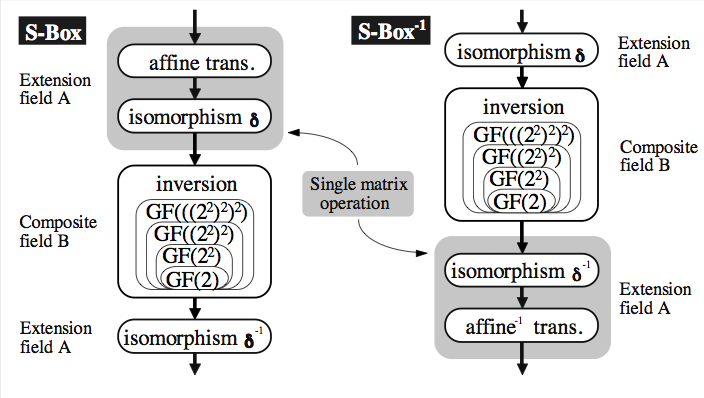
\includegraphics[scale=.35]{./images/tower8bit.png}
	\end{center}
\end{frame}

\section{Hardware Designs}
\subsection{16-Bit S-Boxes}
\begin{frame}
	\frametitle{16-Bit S-Boxes}
	Proposed design - $GF((((2^2)^2)^2)^2)$
	\begin{center}
	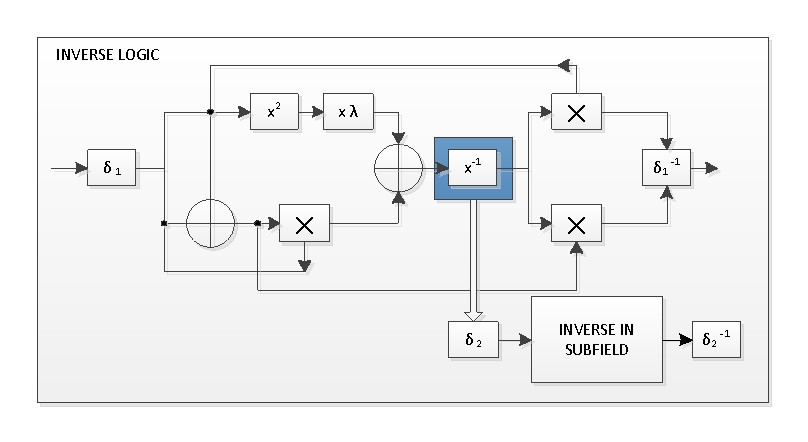
\includegraphics[scale=0.65]{./images/composite_field_inverter.pdf}
	\end{center}
	\textbf{Research question:} How deep should this recession go? What yields the minimal hardware area?
\end{frame}

\begin{frame}
	\frametitle{VHDL Model Overview}
	\begin{itemize}
		\item \textbf{Top-level entity} - SBOX (16-bit input, 16-bit output)
		\begin{itemize}
			\item Internal signals for the input and output of each of the operational blocks
		\end{itemize}
		\item There will be one entity for each multiplicative inverse operation (with the appropriate width I/O signals)
	\end{itemize}	
\end{frame}

\begin{frame}
	\frametitle{What's next?}
	\begin{center}
		Action Items
	\end{center}	
	\begin{itemize}
		\item Hard deadline for VHDL design: \textbf{3/15/13} (sent via email)
		\item Hard deadline for software implementation of isomorphic mapping generation: \textbf{3/16/13} (sent via email) - Python (for simplicity)
		\item Finalized software and scripts to generate vectorial Boolean function representations of S-boxes: \textbf{3/17/13} (sent via email) - combination of C/Python
	\end{itemize}
	\begin{center}
	Next meeting: \textbf{?}
	\end{center}
\end{frame}

\end{document}
